% Time-stamp: <2013-05-25 08:46:53 angenent>
\chapter{Proper and Improper Integrals}%{{{1
All the definite integrals that we have seen so far were of the form
\[
I = \int _a^b f(x) \, \dd x,
\]
where $a$ and $b$ are finite numbers, and where the integrand (the function
$f(x)$) is ``nice'' on the interval $a\leq x\leq b$, i.e.~the function $f(x)$
does not become infinite anywhere in the interval.  There are many situations
where one would like to compute an integral that fails one of these conditions;
i.e.~integrals where $a$ or $b$ is not finite, or where the integrand $f(x)$
becomes infinite somewhere in the interval $a\leq x\leq b$ (usually at an
endpoint).  Such integrals are called \emph{improper integrals. }

If we think of integrals as areas of regions in the plane, then improper
integrals usually refer to areas of infinitely large regions so that some
care must be taken in interpreting them.  The formal definition of the integral
as a limit of Riemann sums cannot be used since it assumes both that the
integration bounds $a$ and $b$ are finite, and that the integrand $f(x)$ is
bounded.  Improper integrals have to be defined on a case by case basis.  The
next section shows the usual ways in which this is done.

\section{Typical examples of improper integrals} %{{{1

\subsection{Integral on an unbounded interval} %{{{2
\label{sec:01improper1}
Consider the integral
\[
A = \int_1^\infty \frac{\dd x} {x^3}.
\]
This integral has a new feature that we have not dealt with before, namely, one
of the integration bounds is ``$\infty$'' rather than a finite number.  The
interpretation of this integral is that it is the area of the region under the
graph of $y=1/x^3$, with $1<x<\infty$.
\begin{center}
  \input ../figures/222/01areaunder-cubichyperbola.pdf_tex
\end{center}
Because the integral goes all the way to ``$x=\infty$'' the region whose area it
represents stretches infinitely far to the right.  Could such an infinitely wide
region still have a finite area?  And if it is, can we compute it?  To compute
the integral $I$ that has the $\infty$ in its integration bounds, we first
replace the integral by one that is more familiar, namely
\[
A_M = \int_1^M \frac{\dd x} {x^3},
\]
where $M>1$ is some finite number.  This integral represents the area of a
finite region, namely all points between the graph and the $x$-axis, and with
$1\leq x\leq M$.
\begin{center}
  \input ../figures/222/01areaunder-cubichyperbola-truncated.pdf_tex
\end{center}
We know how to compute this integral:
\[
A_M = \int_1^M\frac{\dd x} {x^3} =\Bigl[-\frac{1} {2x^2}\Bigr]_1^M = -\frac{1}
{2M^2} + \frac{1} {2}.
\]
The area we find depends on $M$.  The larger we choose $M$, the larger the
region is and the larger the area should be.  If we let $M\to\infty$ then the
region under the graph between $x=1$ and $x=M$ will expand and eventually fill up
the whole region between graph and $x$-axis, and to the right of $x=1$.  Thus
the area should be
\[
A = \lim_{M\to \infty} A_M = \lim_{M\to \infty} \int_1^M \frac{\dd x} {x^3}
=\lim_{M\to\infty} \Bigl[ -\frac{1} {2M^2} + \frac{1} {2} \Bigr] =\frac{1} {2}.
\]
We conclude that the infinitely large region between the graph of $y=1/x^3$ and
the $x$-axis that lies to the right of the line $x=1$ has finite area, and that
this area is exactly~$\frac12$!

\subsection{Second example on an unbounded interval}\label{sec:01improper2} %{{{2
The following integral is very similar to the one we just did:
\[
A = \int _1^\infty \frac{\dd x} {x}.
\]
The integral represents the area of the region that lies to the right of the
line $x=1$, and is caught between the $x$-axis and the hyperbola $y=1/x$.
\begin{center}
  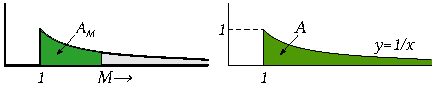
\includegraphics{01areasunderhyperbola.pdf}
\end{center}
As in the previous example the region extends infinitely far to the right while
at the same time becoming narrower and narrower.  To see what its area is we
again look at the truncated region that contains only those points between the
graph and the $x$-axis, and for which $1\leq x\leq M$.  This area is
\[
A_M = \int_1^M \frac{\dd x} {x} = \bigl[\ln x\bigr]_1^M = \ln M - \ln 1 = \ln M.
\]
The area of the whole region with $1\leq x<\infty$ is the limit
\[
A = \lim_{M\to\infty} A_M = \lim_{M\to\infty} \ln M = +\infty.
\]
So we see that the area under the hyperbola is \textbf{not finite!}

\subsection{An improper integral on a finite interval} %{{{2
\label{sec:01improper3}
In this third example we consider the integral
\[
I = \int_0^1 \frac{\dd x} {\sqrt{1-x^2}}.
\]
The integration bounds for this integral are $0$ and $1$ so they are finite, but
the integrand becomes infinite at one end of the integration interval:
\marginpar{\input ../figures/222/01area-is-arcsine.pdf_tex}
\[
\lim_{x\nearrow 1} \frac{1} {\sqrt{1-x^2}} = +\infty.
\]
The region whose area the integral $I$ represents does not extend infinitely far
to the left or the right, but in this example it extends infinitely far upward.
To compute this area we again truncate the region by looking at all points with
$1\leq x\leq a$ for some constant $a<1$, and compute
\[
I_a = \int_0^a \frac{\dd x} {\sqrt{1-x^2}} = \bigl[\arcsin x\bigr]_0^a = \arcsin
a.
\]
The integral $I$ is then the limit of $I_a$, i.e.
\[
\int_0^1\frac{\dd x} {\sqrt{1-x^2}} = \lim_{a\nearrow 1} \int_0^a\frac{\dd x}
{\sqrt{1-x^2}} = \lim_{a\nearrow1} \arcsin a = \arcsin 1 = \frac{\pi} {2}.
\]
We see that the area is finite.


% \subsection{When is an integral improper?} %{{{2
% The definition of the integral
% \[
% \int_a^b f(x) \dd x
% \]
% that was given in first semester calculus (math 221) using Riemann sums assumes
% that the integration interval is finite (i.e.~both $a $nd $b$ are finite
% numbers), and it also assumes that the integrand (the function being integrated)
% is bounded.  If one of these conditions does not hold then the integral is
% called \emph{improper}.  In other words, the integral is improper in either of
% the following two situations:
% \begin{itemize}
% \item \textit{the interval of integration is unbounded} (i.e.~$a=-\infty$ or
%   $b=+\infty$), or

% \item \textit{the function $f(x)$ is not bounded} (this usually happens because
%   $\lim_{x\searrow a} f(x) = \pm\infty$, or $\lim_{x\nearrow b} f(x) =
%   \pm\infty$, or $\lim_{x\to c} f(x) = \pm\infty$ at some other point $c$ in the
%   interval $(a,b)$.)

% \end{itemize}

\subsection{A doubly improper integral}  Let us try to compute %{{{2
\[
I = \int_{-\infty}^\infty \frac{\dd x} {1+x^2}.
\]
This example has a new feature, namely, both integration limits are infinite.
To compute this integral we replace them by finite numbers, i.e.~we compute
\begin{align*}
  \int_{-\infty}^\infty \frac{\dd x} {1+x^2}
  & = \lim_{a\to-\infty} \,\lim_{b\to\infty}
  \int_a^b \frac{\dd x} {1+x^2}\\
  & =  \lim_{a\to-\infty} \,\lim_{b\to\infty} \arctan(b) - \arctan(a) \\
  & = \lim_{b\to\infty} \arctan b  - \lim_{a\to-\infty} \arctan a \\
  & = \frac{\pi} {2} - \bigl(-\frac{\pi} {2}\bigr) \\
  & = \pi.
\end{align*}
{\color{badgerred}\bfseries\textdbend}
A different way of getting the same example is to replace $\infty$ and $-\infty$
in the integral by $a$ and $-a$ and then let $a\to\infty$.  The only difference
with our previous approach is that we now use one variable ($a$) instead of two
($a$ and $b$).  The computation goes as follows:
\begin{align*}
  \int_{-\infty}^\infty \frac{\dd x} {1+x^2}
  &= \lim_{a\to\infty} \int_{-a}^a  \frac{\dd x} {1+x^2} \\
  &= \lim_{a\to\infty} \Bigl(\arctan(a) - \arctan(-a)\Bigr)\\
  &= \frac\pi2 - \bigl(-\frac\pi2\bigr) = \pi.
\end{align*}
In this example we got the same answer using either approach.  This is not
always the case, as the next example shows.
\subsection{Another doubly improper integral} %{{{2
\label{sec:02doubly-improper-xdx}
Suppose we try to compute the integral
\[
I = \int_{-\infty}^\infty x\,\dd x.
\]
The shorter approach where we replace both $\pm\infty$ by $\pm a$ would be
\begin{align*}
  \int_{-\infty}^\infty x\,\dd x
  = \lim_{a\to\infty} \int_{-a}^a x\,\dd x
  = \lim_{a\to\infty} \frac{a^2} {2} - \frac{(-a)^2} {2} 
  = 0.
\end{align*}
On the other hand, if we take the longer approach, where we replace $-\infty$
and $\infty$ by two different constants, then we get this
\begin{align*}
  \int_{-\infty}^\infty x\,\dd x
  &= \lim_{a\to-\infty} \lim_{b\to\infty} \int_{a}^b x\,\dd x\\
  &= \lim_{a\to-\infty} \lim_{b\to\infty} \Bigl[\frac{x^2} {2}\Bigr]\\
  & = \lim_{b\to\infty} \frac{b^2} {2}  - \lim_{a\to-\infty} \frac{a^2} {2}.
\end{align*}
At this point we see that both limits $\lim_{b\to\infty}b^2/2 = \infty$ and
$\lim_{a\to-\infty} a^2/2=\infty$ do not exist.  The result we therefore get is
\[
  \int_{-\infty}^\infty x\,\dd x = \infty - \infty.
\]
Since $\infty$ is not a number we find that the improper integral does not
exist.
\marginpar{\footnotesize\sffamily\color{darkbluegreen}%
  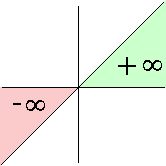
\includegraphics{02improper-xdx.pdf}\\
  $\int_{-\infty}^\infty x\,\dd x$ is the area above minus the area below the axis.}

We conclude that for some improper integrals different ways of computing them
can give different results.  This means that we have to be more precise and
specify which definition of the integral we use.  The next section lists the
definitions that are commonly used.


\section{Summary: how to compute an improper integral} %{{{1

\subsection{How to compute an improper integral on an unbounded interval} By %{{{2
definition the improper integral
\[
\int_a^\infty f(x) \,\dd x
\]
is given by
\begin{equation}
  \label{eq:01improper-integral-def1}
  \int_a^\infty f(x) \,\dd x = \lim_{M\to\infty} \int_a^M f(x)\,\dd x.
\end{equation}
This is how the integral in \S~\ref{sec:01improper1} was computed.

\subsection{How to compute an improper integral of an unbounded function} %{{{2
If the integration interval is bounded, but if the integrand becomes infinite at
one of the endpoints, say at $x=a$, then we define
\begin{equation}
  \label{eq:01improper-integral-def2}
  \int_a^b f(x)\, \dd x = \lim_{s\searrow a} \int_s^bf(x)\,\dd x.
\end{equation}

\subsection{Doubly improper integrals} %{{{2
If the integration interval is the whole real line, i.e.~if we need to compute
the integral
\[
  I = \int_{-\infty}^\infty f(x) \,\dd x,
\]
then we must replace both integration bound by finite numbers and then let those
finite numbers go to $\pm\infty$.  Thus we would first have to compute an
antiderivative of $f$,
\[
F(x) = \int f(x)\,\dd x.
\]
The Fundamental Theorem of Calculus then implies 
\[
I_{a, b} = \int_a^b f(x) \,\dd x = F(b) - F(a)
\]
and we set
\[
I = \lim_{b\to \infty}F(b) - \lim_{a\to-\infty} F(a).
\]
Note that according to this definition we have to compute both limits
separately.  The example in Section~\ref{sec:02doubly-improper-xdx} shows that
it really is necessary to do this, and that computing
\[
\int_{-\infty}^\infty f(x) \dd x = \lim_{a\to\infty} F(a) - F(-a)
\]
can give different results.

In general, if an integral
\[
\int _a ^b f(x)\,\dd x
\]
is improper at both ends we must replace them by $c$, $d$ with $a<c<d<b$ and
compute the limit
\[
\int_a^b f(x) \, \dd x
=
\lim_{c\searrow a} \lim_{d \nearrow b} \int_c^d f(x) \,\dd x.
\]
For instance,
\[
\lim\int_{-1}^1 \frac{\dd x} {\sqrt{1-x^2}}
= \lim_{c\searrow -1}\lim_{d\nearrow 1}
     \int_c^d \frac{\dd x} {\sqrt{1-x^2}}\dots %FINISH THE COMPUTATION
\]

\section{More examples} %{{{1

\subsection{Area under an exponential} Let $a$ be some positive constant and %{{{2
consider the graph of $y= e^{-ax}$ for $x>0$.  How much area is there between
the graph and the $x$-axis with $x>0$?  (See
Figure~\ref{fig:02areasunderexponentials} for the cases $a=1$ and $a=2$.)
\begin{figure}[htb]
  \input ../figures/222/01areaunderexponential.pdf_tex
  \caption{What is the area under the graph of $y=e^{-x}$?  What fraction of
    the region under the graph of $y=e^{-x}$ lies under the graph of
    $y=e^{-2x}$?}
  \label{fig:02areasunderexponentials}
\end{figure}
The answer is given by the improper integral
\begin{align*}
  A &= \int_0^\infty e^{-ax} \,\dd x \\
  &= \lim_{M\to\infty} \int_0^M e^{-ax} \,\dd x \\
  &= \lim_{M\to\infty}\Bigl[-\frac{1} {a}e^{-ax}\Bigr]_0^M\\
  &= -\frac{1} {a}\lim_{M\to\infty} \Bigl( e^{-aM}-1 \Bigr)
       & a>0 \text{ so }\lim_{M\to\infty} e^{-aM} = 0\\
  &= \frac{1} {a}.
\end{align*}
We see that the area under the graph is finite, and that it is given by $1/a$.
In particular the area under the graph of $y=e^{-x}$ is exactly $1$, while the
area under the graph of $y=e^{-2x}$ is exactly half that (i.e.~$1/2$).

\subsection{Improper integrals involving $x^{-p}$} %{{{2
The examples in \S~\ref{sec:01improper1} and \S~\ref{sec:01improper2} are
special cases of the following integral
\[
I = \int_1^\infty \frac{\dd x} {x^p}\;,
\]
where $p>0$ is some constant.  We already know that the integral is $\tfrac12$
if $p=3$ (\S~\ref{sec:01improper1}), and also that the integral is infinite
(does not exist) if $p=1$ (\S~\ref{sec:01improper2}).  We can compute it in the
same way as before,
\begin{align}
  \label{eq:02xpintegral-computation}
  I&=  \lim_{M\to\infty} \int_1^M  \frac{\dd x} {x^p} \\
  &=  \lim_{M\to\infty} \Bigl[\frac{1} {1-p}x^{1-p}\Bigr]_1^M
  & \text{\sffamily\footnotesize assume $p\neq1$} \notag \\
  &=  \frac{1} {1-p}\lim_{M\to\infty} \Bigl(M^{1-p} - 1\Bigr).\notag
\end{align}
At this point we have to find out what happens to $M^{1-p}$ as $M\to\infty$.
This depends on the sign of the exponent $1-p$.  If this exponent is positive,
then $M^{1-p}$ is a positive power of $M$ and therefore becomes infinite as
$M\to\infty$.  On the other hand, if the exponent is negative then $M^{1-p}$ is
a negative power of $M$ so that it goes to zero as $M\to\infty$.  To summarize:
\begin{itemize}
\item If $0<p<1$ then $1-p>0$ so that $\lim_{M\to\infty}M^{1-p}=\infty$;
\item if $p>1$ then $1-p<0$, and
  \[
  \lim_{M\to\infty} M^{1-p} = \lim_{M\to\infty} \frac{1} {M^{p-1}} = 0.
  \]
\end{itemize}
If we apply this to \eqref{eq:02xpintegral-computation} then we find that
\begin{align*}
  \text{if }0<p\leq 1 \text{ then }& \int_1^\infty \frac{\dd x} {x^p} = \infty,\\
  \text{and if } p > 1 \text{ then }& \int_1^\infty \frac{\dd x} {x^p} =
  \frac{1} {p-1}.
\end{align*}

\vfill\newpage
\begin{figure}[h]
  \centering
  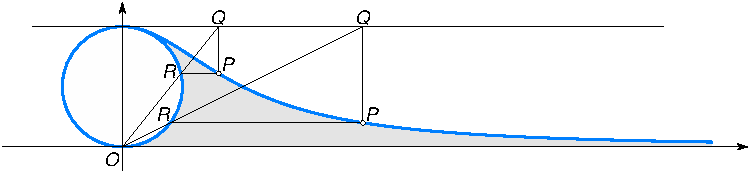
\includegraphics{02Versiera.pdf}
  \caption{{\bfseries Geometric construction of the {\itshape Versiera.}}  The
    figure shows a circle of diameter $1$ that touches the $x$-axis exactly at
    the origin.  For any point $Q$ on the line $y=1$ we can define a new point
    $P$ by intersecting the line segment $OQ$ with the circle, and requiring $P$
    to have the same $x$-coordinate as $Q$ and the same $y$-coordinate as $R$.
    The {\itshape Versiera} is the curve traced out by the point $P$ as we lets
    the point $Q$ slide along the line $y=1$. See problem
    \ref{pblm-area-under-Versiera}. }
  \label{fig:02Versiera}
\end{figure}

\section{Problems} %{{{1
\problemfont %{{{3
\begin{multicols}{2}
\noindent%
Compute the following improper integrals and draw the region whose area they
represent:

\problem $\DS \int_0^\infty \frac{\dd x} {(2+x)^2}$. %{{{3
\answer %{{{3
\begin{align*}
  \int_0^\infty \frac{\dd x} {(2+x)^2}
  &= \lim_{M_\to\infty} \int_0^M \frac{\dd x} {(2+x)^2}\\
  &= \lim_{M\to\infty} \Bigl[\frac{-1} {2+x}\Bigr]_{x=0}^M \\
  &= \lim_{M|to\infty} \Bigl[\frac{-1} {2+M} - \frac{-1} {2+0}\Bigr] \\
  &= \frac{1} {2}.
\end{align*}
\endanswer

\problem $\DS\int_0^{1/2} (2x-1)^{-3}\,\dd x$ %{{{3
\answer %{{{3
The integrand becomes infinite as $x\to\frac{1} {2}$ so this is indeed an
improper integral.
\begin{multline*}
  \int_0^{1/2} (2x-1)^{-3}\,\dd x
  = \lim_{a\nearrow \frac12} \int_{0}^a (2x-1)^{-3} \,\dd x
  = \lim_{a\nearrow \frac12} \Bigl[-\frac14(2x-1)^{-2}\Bigr]_{0}^a\\
  = \lim_{a\nearrow \frac12} -\frac14(2a-1)^{-2} + \frac14 =-\infty.
\end{multline*}
\endanswer

\problem $\DS\int_0^{3} \frac{\dd x}{\sqrt{3-x}}$. %{{{3
\answer %{{{3
The integral is improper at $x=3$:
\[
  \int_0^{3} \frac{\dd x}{\sqrt{3-x}}
  = \lim_{a\nearrow 3} \int_0^{a} \frac{\dd x}{\sqrt{3-x}}
  = \lim_{a\nearrow 3} \Bigl[-2 \sqrt{3-x}\Bigr]_{x=0}^{x=a}
  = \lim_{a\nearrow 3} \Bigl(-2\sqrt{3-a} + 2\sqrt{3-0}\Bigr)
  = 2\surd3.
\]
\endanswer

\problem $\DS\int_0^1 1/\sqrt{x}\,\dd x$. %{{{3
\answer %{{{3
$2$
\endanswer

\problem $\DS \int_0^\infty x e^{-x^2} \,\dd x$. %{{{3
\answer %{{{3
Substitute $u=x^2$ to get the antiderivative
$\int xe^{-x^2}\,\dd x = -\frac12 e^{-x^2}+C$.  The improper integral then is:
\[
\int_0^\infty xe^{-x^2} \,\dd x =
\lim_{M\to\infty} \int_0^M xe^{-x^2} \,\dd x =
\lim_{M\to\infty} \bigl(-\frac12e^{-M^2} + \frac 12 e^{-0^2}\bigr) = \frac 12.
\]
\endanswer
\problem $\DS \int_1^\infty \frac{x-1} {x+x^2}\,\dd x$. %{{{3

\problem $\DS \int_1^\infty \frac{x-1} {x^3+x^2}\,\dd x$. %{{{3

\problem $\DS \int_0^7 \frac{\dd x} {\sqrt{x}}$. %{{{3
\answer %{{{3
$\int_0^7x^{-1/2}\dd x = \lim_{a\searrow 0}\int_a^7 x^{-1/2}\dd x
=\lim_{a\searrow0}\bigl[2x^{1/2}\bigr]_{x=a}^7 = 2\sqrt{7}.$
\endanswer

\problem $\DS \int_0^1 \frac{\dd x} {x\sqrt{x}}$. %{{{3
\answer %{{{3
This integral is infinite.
\endanswer

\problem $\DS \int_0^1 \frac{\dd x} {x+\sqrt{x}}$.\hfill %{{{3
(suggestion: $x=u^2$)

\problem $\DS \int_0^1 \Bigl(\frac{1} {\sqrt{x}} + \frac{1} {x}\Bigr)\,\dd x$. %{{{3

\problem $\DS \int_5^\infty e^{-2x} \,\dd x$ %{{{3
\answer %{{{3
$\frac12 e^{-10}$
\endanswer

\problem $\DS \int_0^\infty x e^{-x}\,\dd x$ %{{{3
\answer %{{{3
$1$
\endanswer

\problem $\DS \int_0^\infty xe^{-x^2}\,\dd x$ %{{{3
\answer %{{{3
$\frac12$.
\endanswer

\problem $\DS \int_0^{\infty} e^{-\sqrt x}\,\dd x$ %{{{3
\answer %{{{3
To do the integral, substitute $x=u^2$.  The answer is $2$.
\endanswer



\problem \label{pblm-area-under-Versiera} The graph of the function %{{{3
$y=1/(1+x^2)$ is called the \textit{Versiera} (see Figure~\ref{fig:02Versiera}).
Compute the area of the shaded region between the Versiera and the circle in
Figure~\ref{fig:02Versiera}.

\problem Let $a$ be a positive constant. %{{{3

\subprob  Draw the graph of $y=xe^{-ax}$, $0\leq x<\infty$ (the function has one
maximum: where is it?)

\subprob Compute $\DS I_a = \int_0^\infty xe^{-ax}\,\dd x$.  How does $I_a$
depend on $a$?

\subprob Compute $\lim_{a\searrow 0} I_a$.  Interpret your answer using the
graphs of $y=x^{-ax}$ that you drew in part (i).

\problem $\DS \int_{-\infty}^0 e^x\, \dd x$.  How would you define this integral %{{{3
(one of the integration bounds is $-\infty$ rather than $+\infty$)?

\problem \subprob $\DS \int_0^\infty e^{-x}\sin \pi x\, \dd x$ where $a,b$ are positive %{{{3
constants.  (You have done the integral before -- see Ch I,
\S~\ref{sec:integration-by-parts-problems},
Problem~\ref{pblm:integral-eax-sinbx} .)

\subprob\carefulnow   As in the previous problems,
draw the region whose area the integral from (\textbf{a}) represents.  Note that
the function in the integral for this problem is not positive everywhere.  How
does this affect your answer?  Can you tell from your drawing if the integral is
positive?  

\problem (\textit{A way to visualize that $\int_1^\infty \frac{\dd x} {x}=\infty$}) %{{{3

\subprob Show that for any $a>0$ one has
\[
\int_a^{2a} \frac{\dd x} {x} = \ln2;
\]
in particular, this integral is the same for all $a>0$.

\subprob Compute the area under the graph of $y=1/x$ between $x=1$ and $x=2^n$
is $n\cdot \ln 2$ by splitting the region into:
\begin{itemize}
\item the part where $1\leq x\leq 2$,
\item the part where $2\leq x\leq 4$,
\item the part where $4\leq x\leq 8$,
\item[$\vdots$]
\item the part where $2^{n-1}\leq x \leq 2^n$.
\end{itemize}
\subprob Explain how the answer to \textbf{(b)} implies that the integral
$\int_1^\infty \dd x/x$ does not exist.

\problem The area under the graph of $y=1/x$ with $1\leq x <\infty$ is infinite. %{{{3
Compute the volume of the funnel-shaped solid you get by revolving this region
around the $x$-axis.  Is the volume of this funnel finite or infinite?
\answer %{{{3
$\int_1^\infty \pi r^2\, \dd x = \pi \int_1^\infty x^{-2}\dd x = \pi$
\endanswer



\end{multicols}
\noproblemfont

\section{Estimating improper integrals} %{{{1
Sometimes it is just not possible to compute an improper integral
because we simply cannot find an antiderivative for the integrand.
\begin{figure}[t]
  \centering \input ../figures/222/02improperintegral-comparison.pdf_tex
  \label{fig:02improper-integral-comparison}
  \caption{\textbf{Comparing improper integrals.  } Here $f$ and $g$ are
  positive functions that satisfy $f(x)\leq g(x)$ for all $x\geq a$.  If
  $\int_a^\infty g(x)\,\dd x$ is finite, then so is $\int_a^\infty f(x)\,\dd x$.
  Conversely, if $\int_a^\infty f(x)\,\dd x$ is not finite, then $\int_a^\infty
  g(x)\,\dd x$ cannot be finite either.}

  \bigskip
  
  \input ../figures/222/01comparison-of-improper-integrals.pdf_tex
  \caption{ In this figure $f(x)$ is again positive, but $g(x)$ is bounded by
  $-f(x)\leq g(x)\leq f(x)$.  The same conclusion still holds, namely, if
  $\int_a^\infty f(x)\dd x$ exists, then so does $\int_a^\infty g(x)\dd x$.}
\end{figure}
When this happens we can still try to estimate the integral by comparing it with
easier integrals, and even if we cannot compute the integral we can still try to
answer the question ``does the integral exist,'' i.e.
\begin{center}
  \itshape Does \ $\DS\lim_{M\to \infty}\int _a^M f(x)\, \dd x$\
  exist?
\end{center}
In this section we will see a number of examples of improper integrals that much
easier to estimate than to compute.  Throughout there are three principles that
we shall use:

\subsubsection*{Integral of a positive function} If the function $f(x)$
satisfies $f(x)\geq 0$ for all $x\geq a$ then either the integral $\int_a^\infty
f(x) \dd x$ exists, or else it is infinite, by which we mean
\[
\lim_{M\to\infty} \int_a^M f(x)\,\dd x = \infty.
\]
If the function $f(x)$ is not always positive then the above limit can fail to
exist by oscillating without ever becoming infinite.  For an example see
\S~\ref{sec:int-to-infty-of-cos}; see also
\S~\ref{sec:improper-integral-of-positive-f} for further explanation.

\subsubsection*{Comparison with easier integrals} If $y=f(x)$ and
$y=g(x)$ are functions defined for $x\geq a$, and if $|g(x)|\leq f(x)$
for all $x\geq a$, then
\[
\left|\int_a^\infty g(x) \;\dd x\right| \leq \int_a^\infty f(x) \;\dd
x.
\]
In particular,
\begin{align*}
  \int_a^\infty f(x)\;\dd x \text{ exists}&\implies
  \int_a^\infty g(x)\;\dd x \text{ exists,} \\
  \int_a^\infty g(x)\;\dd x \text{ does not exist}&\implies
  \int_a^\infty f(x)\;\dd x \text{ does not exist.}
\end{align*}
Read \S~\ref{sec:02comparison-thm} for more details and examples.

\subsubsection*{Only the tail matters} If $f(x)$ is a continuous
function for all $x\geq a$, then for any $b\geq a$ we have
\[
\int_a^\infty f(x)\;\dd x \text{ exists } \iff \int_b^\infty f(x)\;\dd
x \text{ exists.}
\]
Furthermore, for any $b\geq a$ we have
\begin{equation}
  \label{eq:integral-is-beginning-plus-tail}
  \int_a^\infty f(x)\;\dd x = \int_a^b f(x)\;\dd x +\int_b^\infty f(x)\;\dd x.
\end{equation}
This is further explained in Theorem~\ref{thm:tail-of-integral} and the examples
following it.

\subsection{Improper integrals of positive functions} %{{{2
\label{sec:improper-integral-of-positive-f}
Suppose that the function $f(x)$ is defined for all $x\geq a$, and that
$f(x)\geq 0$ for all $x$.  To see if the improper integral $\int_a^\infty
f(x)\,\dd x$ exists we have to figure out what happens to
\[
I_M = \int_a^M f(x)\,\dd x
\]
as $M\nearrow\infty$.  Since we are assuming that $f(x)\geq 0$ the
integral $I_M$ represents the area under the graph of $f$ up to $x=M$.
As we let $M$ increase this region expands, and thus the integral
$I_M$ increases.  So, as $M\nearrow\infty$ there are two
possibilities: either $I_M$ remains finite and converges to a finite
number, or $I_M$ becomes infinitely large.  The following theorem
summarizes this useful observation:

\subsubsection{Theorem}\itshape%
\label{thm:02improper-int-of-pos-function}%
If $f(x)\geq 0$ for all $x\geq a$ then either the integral
\[
I = \int_a^\infty f(x) \, \dd x
\]
exists, (i.e.~$I$ is a finite number), or else
\[
I = \int_a^\infty f(x) \, \dd x = \infty, \quad\text{i.e.}\quad
\lim_{M\to\infty} \int_a^M f(x) \, \dd x =\infty.
\]\upshape

\subsubsection{Example - integral to infinity of the cosine}
\label{sec:int-to-infty-of-cos}
To illustrate what Theorem~\ref{thm:02improper-int-of-pos-function}
says, let's consider an improper integral of a function that is not
always positive. For instance, consider
\[
I = \int_0^\infty \cos x \;\dd x.
\]
The function in the integral is $f(x) = \cos x$, and this function is
clearly not always positive.  When we try to compute this integral we
get
\[
I = \lim_{M\to\infty} \int_0^M \cos x \;\dd x =\lim_{M\to\infty}
\Bigl[\sin x\Bigr]_{x=0}^M =\lim_{M\to\infty} \sin M.
\]
This limit does not exist as $\sin M$ oscillates up and down between
$-1$ and $+1$ as $M\to\infty$.  On the other hand, since $\sin M$
stays between $-1$ and $+1$, we cannot say that
\[
\lim_{M\to\infty} \int_0^M \cos x \;\dd x = +\infty.
\]
Theorem~\ref{thm:02improper-int-of-pos-function} tells us that if we
integrate a positive function then this kind of oscillatory behavior
cannot occur.




\subsection{Comparison Theorem for Improper Integrals} %{{{2
\label{sec:02comparison-thm}\itshape
Suppose $f(x)$ and $g(x)$ are functions that are defined for $a\leq x
<\infty$, and suppose that $|g(x)|\leq f(x)$ for all $x\geq a$, i.e.
\[
-f(x) \leq g(x) \leq f(x) \text{ for all }x\geq a.
\]
If the improper integral $\int_a^\infty f(x)\,\dd x$ exists then the
improper integral $\int_a^\infty g(x)\,\dd x$ also exists, and one has
\[
\left|\int_a^\infty g(x)\;\dd x\right| \leq \int_a^\infty f(x)\;\dd x.
\]\upshape%

This theorem is used in two ways: it can be used to verify that some
improper integral exists without actually computing the integral, and
it can also be used to estimate an improper integral.

\subsubsection{Example}
\label{sec:02first-comparison-example}
Consider the improper integral
\[
I = \int_1^\infty \frac{\dd x} {1+x^3}.
\]
The function in the integral is a rational function so in principle we
know how to compute the integral.  It turns out the computation is not
very easy.  If we don't really need to know the exact value of the
integral, but only want a rough estimate of the integral, then we
could compare the integral with an easier integral.

To decide which simpler integral we should use as comparison, we
reason as follows.  Since ``only the tail matters,'' we consider the
integrand $\frac{1} {1+x^3}$ for large $x$.  When $x$ is very large
$x^3$ will be much larger than $1$, so that we may guess that we can
ignore the ``$1$'' in the denominator $1+x^3$:
\begin{equation}
  \label{eq:one-plusxcubed-approx-xcubed}
  \frac{1} {1+x^3} \approx \frac{1} {x^3} \quad \text{as }x\to\infty.
\end{equation}
This suggests that we may be able to compare the given integral with
the integral
\[
\int_1^\infty \frac{1} {x^3}\;\dd x.
\]
We know from our very first example in this chapter
(\S~\ref{sec:01improper1}) that this last integral is finite (we found
that it is $\frac12$).  Therefore we can guess that our integral $I$
also is finite.

Now let's try to use the Comparison Theorem \ref{sec:02comparison-thm}
to get certainty by proving that the integral $I$ does indeed exist.
We want to show that the integral $\int_1^\infty \frac{1} {1+x^3}\dd
x$ exists, so we choose
\[
g(x) = \frac{1} {1+x^3},\quad \text{and thus } f(x) = \frac{1} {x^3}.
\]
We can compare these functions as follows:
\begin{align*}
  \text{it follows from: }&x^3 \leq 1+x^3 \text{ for all $x\geq 1$} &
  \left(\parbox{78pt}
  {\footnotesize\sffamily divide both sides first by $x^3$ and then by
    $1+x^3$}\right)
  \\
  \text{that: }&\frac{1} {1+x^3} \leq \frac{1} {x^3} \text{ for }x\geq 1 &
\end{align*}
This tells us that
\[
\int_1^\infty \frac{\dd x} {1+x^3} \leq \int_1^\infty \frac{\dd x}
{x^3} =\frac{1} {2}.
\]
Therefore we have found that the integral $I$ does indeed exist, and
that it is no more than~$\frac12$.

We can go beyond this and try to find a \textit{lower bound} (instead
of saying that $I$ is no more than $\frac12$ we try to say that it is
at least as large as some other number.)  Here is one way of doing
that:
\begin{align*}
  &1+x^3 \leq x^3+x^3 \text{ for all }x\geq1\\
  \implies&1+x^3 \leq 2x^3 \text{ for all $x\geq 1$} &
  \left(\parbox{78pt}{\footnotesize\sffamily divide both sides first by
    $2x^3$ and then by $1+x^3$}\right)
  \\
  \implies& \frac{1} {2x^3} \leq \frac{1} {1+x^3} \text{ for }x\geq 1
  &
\end{align*}
This implies that
\[
\int_1^\infty \frac{\dd x} {2x^3} \leq \int_1^\infty \frac{\dd x}
{1+x^3}.
\]
The first integral here is half the integral we computed in
\S~\ref{sec:01improper1}, so we get
\[
\frac{1} {4} \leq \int_1^\infty \frac{\dd x} {1+x^3}.
\]
In summary, we have found that
\[
\frac{1} {4} \leq \int_1^\infty \frac{\dd x} {1+x^3} \leq \frac{1}
{2}.
\]

\subsubsection{Second example}\label{sec:second-comparison-example} Does the
integral
\[
I = \int_1^\infty \frac{x} {x^2+1} \;\dd x
\]
exist?  Since the function we are integrating is positive, we could
also ask \textit{is the integral finite?}

As in the previous example we look at the behavior of the integrand as
$x\to\infty$.  For large $x$ we can assume that $x^2$ is much larger
than $x$, so that it would be reasonable to ignore the $1$ in the
denominator $x^2+1$.  If we do that than we find that
\[
\frac{x} {x^2+1} \approx \frac{x} {x^2} = \frac{1} {x}.
\]
If this were correct, then we would end up comparing the integral $I$
with the simpler integral
\[
\int_1^\infty \frac{1} {x}\; \dd x.
\]
We know this latter integral is not finite (it was our second example,
see \S~\ref{sec:01improper2}) and therefore we guess that the integral
$I$ probably also is not finite.  To give a sound argument we will use
the Comparison Theorem.

Our goal is to show that the integral
\[
I = \int_1^\infty f(x)\;\dd x, \quad \text{with } f(x) = \frac{x}
{1+x^2}
\]
is not finite.  To do this we have to find a function $g(x)$ such that
\begin{itemize}
\item $g(x)$ is smaller than $f(x)$ (so that $\int f \dd x$ will be
  larger than $\int g(x)\dd x$),
\item $g(x)$ is easy to integrate, and
\item the integral of $g(x)$ is not finite.
\end{itemize}
The first and last point together imply that
\[
I = \int_1^\infty f(x)\;\dd x \geq \int_1^\infty g(x)\;\dd x =\infty,
\]
which is what we are trying to show.

To complete the reasoning we have to find the easy-to-integrate
function $g(x)$.  Based on what we have done above our first guess
would be $g(x) = \frac{1} {x}$, but this does not work, since
\[
\frac{x} {x^2+1} < \frac{x} {x^2} = \frac{1} {x}.
\]
So with this choice of $g(x)$ we get $g(x)>f(x)$ instead of
$g(x)<f(x)$.

One way to simplify $f(x)$ and get a smaller function is to remember
that \textit{by increasing the denominator in a fraction we decrease
  the fraction}.  Thus, for $x>1$ we have
\[
f(x) = \frac{x} {x^2+1} > \frac{x} {x^2 + x^2} = \frac{x} {2x^2} =
\frac{1} {2x}.
\]
So we let $g(x) = \frac{1} {2x}$.  Then we find
\begin{align*}
  I
  &= \int _1^\infty \frac{x} {x^2+1} \;\dd x\\
  &\geq \int _1^\infty \frac{1} {2x} \;\dd x\\
  & = \infty.
\end{align*}


\subsection{The Tail Theorem}\label{thm:tail-of-integral}\itshape% %{{{2
If $y=f(x)$ is a continuous function for $x\geq a$, and if $b>a$ then
\[
\int_a^\infty f(x) \;\dd x \text{ exists if and only if }
\int_b^\infty f(x) \;\dd x \text{ exists }
\]
Moreover, if these integrals exist, then
\eqref{eq:integral-is-beginning-plus-tail} holds: $\int_a^\infty
f(x)\,\dd x = \int_a^b f(x)\,\dd x + \int_b^\infty f(x)\,\dd
x$.\upshape

\medskip
\begin{proof}
  For any finite $M$ one has
  \[
  \int_a^M f(x)\,\dd x = \int_a^b f(x)\,\dd x + \int_b^M f(x)\,\dd x
  \]
  The theorem follows by taking the limit for $M\to\infty$ on both
  sides of this equation.
\end{proof}

The following two examples show how one can use this fact.

\subsubsection{Example}
\itshape%
Does the integral
\[
I = \int_0^\infty \frac{\dd x} {x^3+1}
\]
exist?\upshape

The integrand here is the same as in \S~\ref{sec:02first-comparison-example}
where we found that
\[
\int_1^\infty \frac{\dd x} {x^3+1} < \frac12,
\]
and in particular is finite.  Since the function $f(x) = 1/(x^3+1)$ is
continuous for $0\leq x\leq 1$ we may conclude that
\[
I = \int_0^\infty \frac{\dd x} {x^3+1}
=
\int_0^1 \frac{\dd x} {x^3+1} +
\int_1^\infty \frac{\dd x} {x^3+1}
\]
so that $I$ is finite.

If we want an upper estimate for the integral we can use the fact that we
already know that the integral from $1$ to $\infty$ is not more than $\frac12$
and estimate the integral from $x=0$ to $x=1$.  For $0\leq x\leq 1$ we have
\[
x^3+1 \geq 1 \implies \frac{1} {x^3+1} \leq 1
\]
This implies
\[
\int_0^1 \frac{\dd x} {x^3 + 1} \leq \int _0^1 1\, \dd x =1,
\]
and hence
\[
\int_0^\infty\frac{\dd x} {x^3 + 1} =
\int_0^1 \frac{\dd x} {x^3+1} +
\int_1^\infty \frac{\dd x} {x^3+1}
\leq 1+ \frac{1} {2} = \frac{3} {2}.
\]


\subsubsection{The area under the bell curve}
\label{sec:01area-under-bell-curve}
The \emph{bell curve} which plays a central role in probability and statistics,
is the graph of the function
\[
n(x) = a e^{-x^2/b},
\]
where $a$ and $b$ are positive constants whose values will not be important in
this example.  In fact, to simplify this example we will choose them to be $a=1$
and $b=1$ so that we are dealing with the function $n(x) = e^{-x^2}$.  The
question now is, \textit{is the area under the bell curve finite, and can we
estimate it?}  In terms of improper integrals, we want to know if the integral
\[
A = \int_{-\infty}^\infty e^{-x^2}\;\dd x
\]
exists.

\begin{figure}[b]
  \centering \input ../figures/222/01area-under-bell-curve.pdf_tex
  \caption{Estimating the area under the bell curve.}
  \label{fig:area-under-bell-curve}
\end{figure}


We write the integral as the sum of two integrals
\[
\int_{-\infty}^\infty e^{-x^2}\;\dd x = \int_{-\infty}^0 e^{-x^2}\;\dd
x + \int_{0}^\infty e^{-x^2}\;\dd x
\]
Since the function $n(x) = e^{-x^2}$ is even\marginpar{\footnotesize\sffamily
  $n(x)=n(-x)$ so the bell curve is symmetric} these two integrals are equal, so
if we can show that one of them exists, the other will also exist.

When $x$ is large $x^2$ is much larger than $x$ so that $e^{-x^2}$ will be
smaller than $e^{-x}$; since $e^{-x}$ is a function we know how to integrate it
seems like a good idea to compare the bell curve with the graph of $e^{-x}$.  To
make the comparison (and to use the Comparison Theorem) we first check if
$e^{-x^2} \leq e^{-x}$ really is true.  We find that this is true if $x\geq 1$,
namely:
\[
x\geq 1 \implies x^2\geq x \implies -x^2\leq -x \implies e^{-x^2} \leq
e^{-x}.
\]
We can therefore use $e^{-x}$ to estimate the integral of $e^{-x^2}$ for $x\geq
1$:
\[
\int_1^\infty e^{-x^2}\;\dd x \leq \int_1^\infty e^{-x}\;\dd x
=\lim_{M\to\infty} \Bigl[-e^{-x}\Bigr]_1^M =\lim_{M\to\infty}
\bigl(-e^{-M}+e^{-1}\bigr) = e^{-1}.
\]
Between $x=0$ and $x=1$ we have $e^{-x^2} \leq 1$, so
\[
\int_0^1 e^{-x^2}\; \dd x \leq \int_0^1 1\;\dd x = 1,
\]
and therefore
\[
\int_0^\infty e^{-x^2}\;\dd x = \int_0^1 e^{-x^2}\;\dd x +
\int_1^\infty e^{-x^2}\;\dd x \leq 1+\frac{1} {e}.
\]
Since the bell curve is symmetric, we get the same estimates for the integral
over $-\infty<x\leq 0$:
\[
\int_{-\infty}^0 e^{-x^2}\;\dd x \leq 1+\frac{1} {e}.
\]
In the end we have shown that the area under the bell curve is finite, and that
it is bounded by
\[
A = \int_{-\infty}^\infty e^{-x^2}\;\dd x \leq 2 + \frac{2} {e}.
\]
With quite a bit more work, and using an indirect argument one can actually
compute the integral (without finding an antiderivative of $e^{-x^2}$).  The
true value turns out to be
\[
A = \int_{-\infty}^\infty e^{-x^2}\;\dd x = \sqrt{\pi}.
\]
For comparison,
\[
\sqrt{\pi} \approx 1.772\,453\,850\,9\ldots \text{ and } 2 + \frac{2}
{e} \approx 2.735\,758\,882\,3\ldots.
\]
%\newpage
\section{Problems} %{{{1
\problemfont %{{{3
\begin{multicols}{2}
\noindent%
Which of the following inequalities are true for all $x>a$ (you get to
choose $a$):

\problem $\DS \frac{1} {x} > \frac{1} {x^2}$?\\ %{{{3
%
\color{darkbluegreen}\textit{Answer: }%{{{3
\textsl{True. If $x>1$ then $x^2 > x$ and therefore $\frac{1} {x^2} < \frac{1}
{x}$.  So the inequality is true if $x>a$ where we choose $a=1$.}
\color{black}

\problem $\DS\frac{1} {x-1} < \frac{1} {x}$\,? %{{{3

\problem $\DS\frac{x} {x^2+2x} > \frac{1} {x}$\,? %{{{3

\answer %{{{3
$\DS\frac{x} {x^2+2x} = \frac{1} {x+2} < \frac{1} {x}$ for all $x>0$, so ``False.''
\endanswer

\problem $\DS\frac{x}{\sqrt{x^3-1}} > x^{-1/2}$\,? %{{{3

\answer %{{{3
True
\endanswer

\problem $\DS\frac{2x^2 - 3x + 1} {(x^2-x)^3} < 2x^{-4}$\,? %{{{3

\answer %{{{3
False.
\endanswer

\smallskip

\centerline{\rule{96pt}{1pt}}
\smallskip


\noindent%
Which of the following inequalities are true for all $x$ with $0<x<a$ (you get to
choose $a$ again, as long as $a>0$):

\problem $\DS \frac{3} {x} > \frac{3} {x^2}$?\\ %{{{3
%
\color{darkbluegreen}\textit{Answer: }%{{{3
\textsl{False. If $0<x<1$ then $x^2 < x$ and therefore $\frac{1} {x^2} > \frac{1}
{x}$, which implies $\frac{3} {x^2} > \frac{3} {x}$.  So, more precisely, the
inequality is false if $0<x<a$ where we choose $a=1$.}
\color{black}

\problem $\DS \frac{x} {x^2+x} < \frac{1} {x}$? %{{{3
%
\answer %{{{3
True because $\frac{x} {x^2+1} = \frac{1} {x+1}$.  For $x>0$ it is always true
that $x+1>x$ and therefore $\frac{1} {x} < \frac{1} {x+1}$ is true for all $x>0$.
\endanswer

\problem $\DS \frac{2} {x-x^2}  < \frac{2} {x}$? %{{{3
%
\answer %{{{3
False.
\endanswer

\problem $\DS \frac{2} {x+x^2}  < \frac{2} {x}$? %{{{3
%
\answer %{{{3
True.
\endanswer

\problem $\DS \frac{4} {x+20x^2}  < \frac{2} {x}$? %{{{3
%
\answer %{{{3
False.
\endanswer

\problem $\DS \frac{2} {x-x^2}  < \frac{4} {x}$? %{{{3
%
\answer %{{{3
True.
\endanswer

\smallskip

\centerline{\rule{96pt}{1pt}}
\smallskip

\noindent%
For each of the following improper integrals draw the graph of the
integrand, and decide if the integral exists.  If it does try to find an
estimate for how large the integral is.

\problem $\DS \int_0^\infty \frac{u^2} {\bigl(u^2+1\bigr)^2}\,\dd u$ %{{{3
%
\answer %{{{3
The integrand is $f(u) = \frac{u^2} {(u^2+1)^2}$, which is continuous at all
$u\geq 0$.  Therefore the integral is improper at $u\to\infty$, but nowhere else.

To determine if the integral converges we may therefore look at ``the tail,''
i.e. we can look at
\[
  I = \int_1^\infty \frac{u^2} {\bigl(u^2+1\bigr)^2} \dd u
\]
instead of the integral starting at $u=0$.

For all $u$ we have $1+u^2 \geq u^2$, and therefore 
\[
  \frac{u^2}{\bigl(1+u^2\bigr)^2} \leq \frac{u^2}{(u^2)^2} = \frac{1}{u^2}.
\]
Therefore
\[
  \int_1^\infty \frac{u^2}{\bigl(1+u^2\bigr)^2} \dd u
  \leq \int_1^\infty \frac{\dd u}{u^2} = 1. \tag{\dag}
\]
This implies for the integral in the problem that
\[
  \int_0^\infty\frac{u^2}{\bigl(1+u^2\bigr)^2}\dd u <\infty.
\]
In other words the integral converges.  To get an actual estimate for how big
the integral is we already have (\dag), so we need to estimate the integral for
$0<u<1$.  On this interval we have
\[
  \frac{u^2}{\bigl(1+u^2\bigr)^2} \leq \frac{u^2}{(1)^2} = u^2,
\]
so that 
\[
  \int_0^1 \frac{u^2}{\bigl(1+u^2\bigr)^2} \dd u
  \leq \int_0^1 u^2\,\dd u = \frac{1}{3}. \tag{\ddag}
\]
Therefore
\[
  \int_0^\infty \frac{u^2}{\bigl(1+u^2\bigr)^2} \dd u
  =
  \int_0^1 \frac{u^2}{\bigl(1+u^2\bigr)^2} \dd u
  +
  \int_1^\infty \frac{u^2}{\bigl(1+u^2\bigr)^2} \dd u
  \leq \frac{1}{3} + 1
  =\frac{4}{3}.
\]

\endanswer

\problem $\DS \int_0^\infty \frac{u^3} {\bigl(u^2+1\bigr)^2}\,\dd u$ %{{{3
%
\answer %{{{3
For large values of $u$ the integrand is approximately given by
\[
  \frac{u^3} {\bigl(u^2+1\bigr)^2} \approx \frac{u^3}{(u^2)^2} = \frac{1}{u}.
\]
Since the integral $\int_1^\infty \frac{\dd u}{u}$ diverges, we expect the
integral $I$ to diverge too.  To confirm this we try to ``estimate the tail from
below.''

For $u>1$ we have 
\[
  1+u^2 < 2u^2,
\]
which implies
\[
\frac{u^3} {\bigl(u^2+1\bigr)^2} >
\frac{u^3}{(2u^2)^2} =  \frac{1}{4u}.
\]
Therefore
\[
  \int_1^\infty \frac{u^3} {\bigl(u^2+1\bigr)^2} \dd u \geq 
  \int_1^\infty \frac{\dd u}{4u} =\infty.
\]
It follow that
\[
  \int_0^\infty \frac{u^3} {\bigl(u^2+1\bigr)^2}\dd u
  =
  \int_0^1\frac{u^3} {\bigl(u^2+1\bigr)^2}\dd u
  +
  \int_1^\infty\frac{u^3} {\bigl(u^2+1\bigr)^2}\dd u
  \geq
  \int_1^\infty \frac{\dd u}{4u} =\infty.
\]
In other words the integral in the problem diverges.

\endanswer

\problem $\DS \int_0^\infty \frac{u^4} {\bigl(u^2+1\bigr)^2}\,\dd u$ %{{{3

\problem $\DS \int_\pi^\infty \frac{\sin x} {x^2}\,\dd x$ %{{{3

\problem $\DS \int_0^\infty \frac{\sin(x^2)} {x^2}\,\dd x$\hfill %{{{3
\parbox{60pt}{\flushright(what happens at $x=0$?)}


\problem\groupproblem  (\textit{Fresnel integrals from optics.}) %{{{3
For background on Fresnel integrals read the Wikipedia article on the subject.

\noindent%
Consider the function $\DS F(x) = \frac{\sin x^2} {2x}$.

\subprob Compute $\DS\lim_{x\to0} F(x)$ and $\DS \lim_{x\to\infty} F(x)$.

\subprob Show that $\DS F'(x) = \cos x^2 - \frac{\sin x^2} {2x^2}$.

\subprob Show that the integral $\DS \int_0^\infty \frac{\sin x^2} {2x^2}\dd x$ exists.

\subprob Show that
\[
\int_0^\infty \cos x^2\;\dd x = \int_0^\infty \frac{\sin
x^2} {2x^2}\dd x.
\]

\subprob True or False: \textit{if for some function $f$ the improper integral
$\int_0^\infty f(x)\, \dd x$ exists then it must be true that $\lim_{x\to\infty}
f(x) =0$?}

\problem\groupproblem  Suppose %{{{3
\[
p(x) = e^{-ax},
\]
where $a>0$ is a constant.

\subprob Show that $\int_0^\infty p(x)\,\dd x<\infty$.  (hint:
you can compute the integral.)

\subprob Compute
\[
\frac{\int_0^\infty x p(x)\, \dd x} {\int_0^\infty p(x)\,\dd x}
\]
by integrating by parts in the integral in the numerator.

\subprob Compute
\[
\frac{\int_0^\infty x^2 p(x)\, \dd x} {\int_0^\infty p(x)\,\dd x}
\]
by integrating by parts twice in the integral in the numerator.

\problem\groupproblem Suppose %{{{3
\[
p(x) = e^{-x^2/\sigma^2}
\]
where $\sigma>0$ is a constant.\\
{\footnotesize\sffamily($\sigma$ is the
Greek lower case ``s,'' pronounced as ``sigma.'')}

\subprob Show that $\int_{-\infty}^\infty p(x)\, \dd x<\infty$.  (hint:
 there is no antiderivative of $e^{-x^2/\sigma^2}$, so don't look for it.
Instead follow example \ref{sec:01area-under-bell-curve}.)

\subprob Compute
\[
\frac{\int_{-\infty}^\infty x p(x)\, \dd x} {\int_0^\infty p(x)\,\dd x}.
\]
Hint: there is an easy antiderivative for the integral in the numerator.  Do
that one first.

\subprob Compute
\[
\frac{\int_{-\infty}^\infty x^2 p(x)\, \dd x} {\int_0^\infty p(x)\,\dd x}
\]
by integrating by parts in the integral in the numerator.

\problem\groupproblem %{{{3

\begin{center}\itshape
  ``The area under the bell curve\\
  is $\frac12$-factorial''
\end{center}
In this problem we look at a new function $F(n)$.  For any number $n$ we
would like to define
\[
F(n) = \int_0^\infty t^n e^{-t}\,\dd t.
\]
The integral that defines $F(n)$ is improper so it is not automatically clear
that $F(n)$ exists.

\subprob Show that the integral exists if $n\geq0$.

\subprob Compute $F(0)$, $F(1)$, and $F(2)$.

\subprob Use integration by parts to show that $F(n+1) = (n+1) F(n)$ Holds for
any $n\geq 0$.  Use this to Compute $F(10)$.

\subprob  If you set $n=-1$ in the relation $F(n+1) = (n+1) F(n)$ then you get
$F(0) = 0\cdot F(-1) = 0$.  This should contradict the value for $F(0)$ you found
in \textbf{(b)}.  What is wrong?

\subprob Show that the integral for $F(\frac12)$ exists, and use a substitution
to show that
\[
F(\tfrac12) = \int_{-\infty}^\infty e^{-u^2} \,\dd u.
\]
How does this justify the statement at the beginning of the problem?


\end{multicols}
\noproblemfont
